\documentclass[12pt,a4paper]{article}
\usepackage[utf8]{inputenc}
\usepackage[T1]{fontenc}
\usepackage[polish]{babel}
\usepackage{graphicx}
\usepackage{xcolor}
\usepackage{listings}
\usepackage{amsmath}
\usepackage{amssymb}
\usepackage{geometry}
\usepackage{fancyvrb} % For Verbatim environment with options if needed

\geometry{a4paper, margin=1in}

% Define colors
\definecolor{darkgreen}{rgb}{0.0, 0.4, 0.0}

% Listings configuration for GTL
\lstdefinestyle{GTLstyle}{
    basicstyle=\ttfamily\color{darkgreen}\small,
    breaklines=true,
    frame=tb, % Top and bottom frame for code blocks
    framesep=5pt,
    framerule=0.5pt,
    rulecolor=\color{black},
    backgroundcolor=\color{white},
    aboveskip=1.0\baselineskip, % Adjusted spacing
    belowskip=1.0\baselineskip, % Adjusted spacing
    columns=flexible,
    keepspaces=true, % Important for GTL's "> " prefix
    literate={>}{{\textgreater}}1 { }{{\textvisiblespace}}1, % Show > and spaces if needed (optional)
    showstringspaces=false, % Do not mark spaces in strings
}
\lstset{style=GTLstyle}

\title{Memecoding (memokod) \\ \large Wprowadzenie i poradnik do języka programowania GTL}
\author{Mateusz Kotarba \\ Juliusz Kociński \\ Jakub Kierznowski}
\date{} % No date to make it timeless

\begin{document}

% --- TITLE PAGE ---
\begin{titlepage}
    \centering
    \vspace{1.5cm}
    {\large Mateusz Kotarba \\ Juliusz Kociński \\ Jakub Kierznowski\par}
    \vspace*{\stretch{0.5}} % Adjust spacing
    {\Huge\bfseries Memecoding\par}
    \vspace{0.5cm}
    {\Large\bfseries Wprowadzenie i poradnik do języka programowania GTL\par}
    \vspace{1.5cm}

    \IfFileExists{img/logo_main_light.jpg}{
        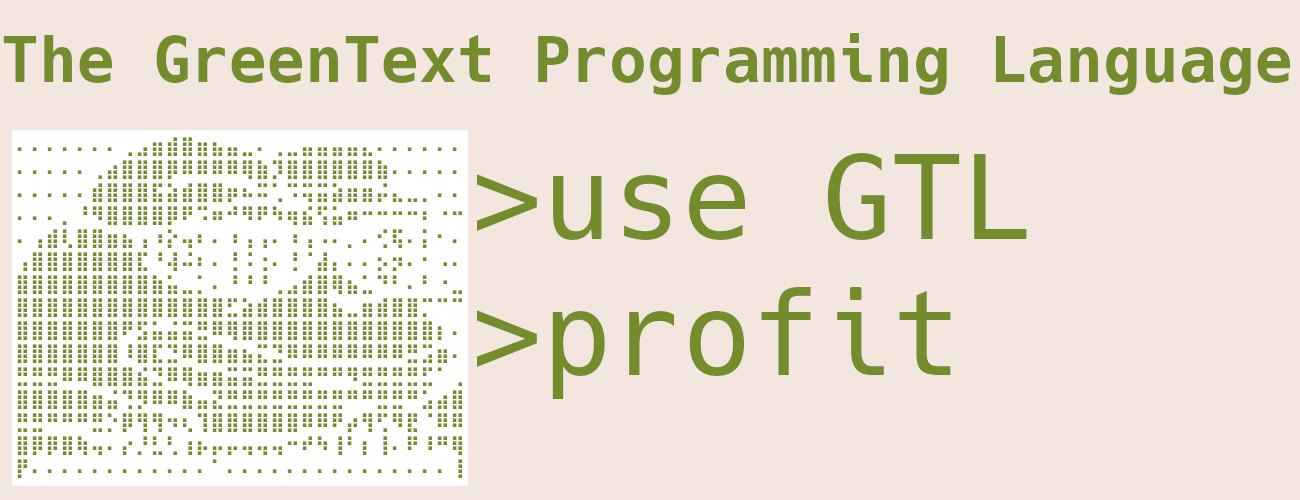
\includegraphics[width=1\textwidth]{img/logo_main_light.jpg}\par
    }{
        \fbox{\parbox[c][8cm][c]{0.5\textwidth}{\centering\Large Logo GTL}}\par % Placeholder
    }
    \vspace*{\stretch{1.5}} % Adjust spacing
    {\small Opracowane na podstawie dokumentacji projektu GTL w ramach kursu "Kompilatory i Teoria Kompilacji \\
    \copyright WEAIiIB AGH 2025 \par}
\end{titlepage}

\tableofcontents
\newpage

% --- CONTENT SECTIONS ---

\section{Wstęp do GreenTextLang (GTL)}
\label{sec:introduction}
GreenText Programming Language (GTL) to wieloparadygmatowy język programowania zaprojektowany tak, aby pisanie w nim kodu przypominało tworzenie klasycznych internetowych historyjek w formacie "green text", spopularyzowanych przez portale takie jak 4chan. GTL, mimo że jest w pełni funkcjonalnym językiem, został stworzony głównie dla zabawy i unikalnego doświadczenia programistycznego, a niekoniecznie do tworzenia kodu produkcyjnego.

Język GTL jest implementowany w Javie przy użyciu ANTLR4. Wiele zaawansowanych funkcji i łatwość użycia zostały czasem poświęcone na rzecz podobieństwa do oryginalnego stylu green text.

\subsection{Główna zasada GTL}
\label{ssec:main_property}
Każda linia kodu w GTL musi być rozpoczęta sekwencją znaków: \textbf{spacja}, znak \textbf{\texttt{>}}, a następnie \textbf{co najmniej jedna spacja}.
Na przykład:
\begin{lstlisting}
 > to jest poprawna linia kodu GTL
\end{lstlisting}

\subsection{Hello World}
\label{ssec:hello_world}
Tradycyjny program "Hello, World!" w GTL może wyglądać następująco:
\begin{lstlisting}
 > spit "Hello, World!"
\end{lstlisting}
Co wyświetli na ekranie:
\begin{verbatim}
Hello, World!
\end{verbatim}

Jeśli chcemy od razu nadać mu formę historyjki (np. w głównej funkcji programu, która często nazywa się `me`):
\begin{lstlisting}
 > be me
 > spit "Hello, World!"
 > profit
\end{lstlisting}
Ten program również wyświetli:
\begin{verbatim}
Hello, World!
\end{verbatim}
Jednakże kluczowa linia będzie zamknięta w funkcji głównej.

\subsubsection*{Ćwiczenie}
Spróbuj napisać program, który wyświetli Twoje imię na ekranie.

\newpage
\section{Czytanie i Wyświetlanie Danych (Input/Output)}
\label{sec:input_output}
GTL umożliwia interakcję z programem poprzez czytanie danych z standardowego wejścia (stdin) oraz wypisywanie danych na standardowe wyjście (stdout).

\subsection{Czytanie z stdin: \texttt{swallow}}
Polecenie \texttt{ > swallow {nazwa\_zmiennej}} służy do czytania danych wprowadzonych przez użytkownika. GTL próbuje automatycznie skonwertować wprowadzone dane na odpowiedni typ danych, jeśli to możliwe. Domyślnie dane są traktowane jako tekst (string).

\subsection{Wypisywanie na stdout: \texttt{spit}}
Do wypisywania danych na ekran używamy polecenia \texttt{ > spit {wartość\_lub\_zmienna}}. Wartości są konwertowane na tekst (jeśli nim nie są) i wyświetlane.

\textbf{Przykład użycia \texttt{spit} i \texttt{swallow}:}
\begin{lstlisting}
 > be io_example
 > # Przyklad 1: Czytanie i wypisywanie tekstu
 > hear user_name
 > spit "Jak masz na imie?"
 > swallow user_name # Program czeka na wpisanie danych
 > spit "Witaj, "
 > spit user_name
 > spit "!"

 > # Przyklad 2: Czytanie liczby i operacja
 > see number_in
 > spit "Podaj liczbe, a ja pomnoze ja przez 2:"
 > swallow number_in
 > see result is number_in breeding like 2 times
 > spit "Wynik to: "
 > spit result
 > profit
\end{lstlisting}
\textbf{Oczekiwany wynik programu (zakładając wpisanie "Tester" i potem 21):}
\begin{verbatim}
Jak masz na imie?
Tester
Witaj,
Tester
!
Podaj liczbe, a ja pomnoze ja przez 2:
21
Wynik to:
42
\end{verbatim}
W przypadku, gdy interaktywne wprowadzanie danych przez \texttt{swallow} nie jest dostępne lub podczas testowania skryptów, dane wejściowe można zasymulować, np. przekazując je do programu przez standardowe wejście (piping) lub modyfikując kod tak, by zmienne były inicjalizowane bezpośrednio.

\subsubsection*{Ćwiczenie}
Napisz program, który:
\begin{enumerate}
    \item Prosi użytkownika o podanie jego ulubionego koloru (użyj \texttt{spit} do wyświetlenia prośby).
    \item Wczytuje odpowiedź do zmiennej typu \texttt{hear} (użyj \texttt{swallow}).
    \item Prosi użytkownika o podanie jego szczęśliwej liczby (użyj \texttt{spit}).
    \item Wczytuje liczbę do zmiennej typu \texttt{see} (użyj \texttt{swallow}).
    \item Wyświetla komunikat: "Twój ulubiony kolor to [kolor], a Twoja szczęśliwa liczba to [liczba]." (użyj \texttt{spit}).
\end{enumerate}
Pamiętaj, aby symulować wprowadzanie danych przez przypisanie, jeśli testujesz w środowisku bez interaktywnego wejścia lub jeśli \texttt{swallow} nie działa interaktywnie w Twoim interpreterze.

\newpage
\section{Zmienne i Typy Danych}
\label{sec:variables}
W GTL zmienne deklaruje się używając specyficznych słów kluczowych odpowiadających typom danych. Słowa kluczowe te odpowiadają różnym zmysłom i doświadczeniom:

\subsection{Podstawowe typy danych}
\begin{itemize}
    \item \texttt{see}: dla liczb całkowitych (integer).
    \item \texttt{taste}: dla liczb zmiennoprzecinkowych (double).
    \item \texttt{hear}: dla ciągów znaków (string).
    \item \texttt{smell}: dla wartości logicznych (boolean).
    \item \texttt{spot}: dla struktur danych (structs).
\end{itemize}

\subsection{Deklarowanie i przypisywanie wartości}
Zmienną deklaruje się według schematu: \texttt{ > {typ} {nazwa} is {wartość}}. Słowo kluczowe \texttt{is} służy do przypisania wartości. Jeśli wartość nie jest podana, zmienna zostanie zainicjalizowana wartością domyślną dla danego typu.

\textbf{Przykłady deklaracji zmiennych:}
\begin{lstlisting}
 > be example_vars
Deklaracja liczby calkowitej
 > see my_age is 25
Deklaracja liczby zmiennoprzecinkowej
 > taste pi_value is 3.14159
Deklaracja ciagu znakow
 > hear greeting is "Witaj w GTL!"
Deklaracja wartosci logicznej
 > smell is_gtl_fun is c: # c: oznacza true

 > spit my_age
 > spit pi_value
 > spit greeting
 > spit is_gtl_fun
 > profit
\end{lstlisting}
\textbf{Oczekiwany wynik programu:}
\begin{verbatim}
25
3.14159
Witaj w GTL!
c:
\end{verbatim}

\subsection{Konwersja Typów (Casting)}
\label{ssec:casting}
GTL obsługuje zarówno jawną, jak i niejawną konwersję typów.

\subsubsection{Jawne Castowanie (Eksplicytne)}
Jawne rzutowanie typów wykonuje się za pomocą frazy \texttt{let me}.
\begin{itemize}
    \item \textbf{Składnia:} \texttt{let me <typ> <wyrażenie\_atom>}
    \item \textbf{Działanie:} Konwertuje wartość wynikającą z \texttt{<wyrażenie\_atom>} na określony \texttt{<typ>}.
    \item \textbf{Przykłady w GTL:}
    \begin{lstlisting}
 > be explicit_cast_example
 > # Rzutuje string "123" na typ see (integer)
 > see my_int is let me see "123"
 > spit my_int

 > hear num_str is "45.67"
 > # Rzutuje string num_str na typ taste (double)
 > taste my_double is let me taste num_str
 > spit my_double
 > profit
    \end{lstlisting}
    \textbf{Oczekiwany wynik programu:}
    \begin{verbatim}
123
45.67
    \end{verbatim}
\end{itemize}

\subsubsection{Niejawne Castowanie (Automatyczne)}
GTL często wykonuje niejawne konwersje typów w następujących sytuacjach:
\begin{itemize}
    \item \textbf{Przypisania do zmiennych:} Gdy przypisujesz wartość do istniejącej zmiennej, GTL próbuje automatycznie skonwertować przypisywaną wartość do typu zmiennej.
    \item \textbf{Przypisania do elementów tablicy:} Wartość jest automatycznie konwertowana do typu elementów tablicy.
    \item \textbf{Operacje arytmetyczne i logiczne:} Typy mogą być promowane lub konwertowane, aby umożliwić operację (np. int do double w operacji z double). Jeśli konwersja nie jest możliwa, może zostać rzucony błąd.
    \item \textbf{Przekazywanie argumentów do funkcji:} Argumenty są konwertowane do typów oczekiwanych przez parametry funkcji.
\end{itemize}
\textbf{Przykład niejawnego castingu (w operacjach):}
\begin{lstlisting}
 > be implicit_cast_example
 > see int_val is 10
 > taste dbl_val is 5.5
 > # int_val zostanie niejawnie rzutowany na double
 > # przed operacja dodawania
 > taste result is int_val joined by dbl_val
 > spit result # Wynik: 15.5
 > profit
\end{lstlisting}
\textbf{Oczekiwany wynik programu:}
\begin{verbatim}
15.5
\end{verbatim}

\subsection{Kolekcje (Tablice)}
GTL wspiera tablice statyczne i dynamiczne.
\begin{itemize}
    \item \texttt{about}: Słowo kluczowe używane przy deklaracji tablicy o stałym rozmiarze. Po \texttt{about} podaje się wyrażenie określające rozmiar.
    \item \texttt{multiple}: Słowo kluczowe używane przy deklaracji tablicy dynamicznej.
\end{itemize}

\textbf{Przykład deklaracji tablic:}
\begin{lstlisting}
 > be example_arrays
Tablica statyczna 5 liczb calkowitych
 > see about 5 numbers is 1, 2, 3, 4, 5
Tablica dynamiczna stringow
 > hear multiple names is "Anon", "Pepe", "Wojak"

Dostęp do elementu tablicy (indeksowanie od 0)
 > spit numbers'th 0 # Wyswietli pierwszy element
 > spit names'th 1   # Wyswietli drugi element

Modyfikacja elementu tablicy
 > names'th 1 is "Chad"
 > spit names'th 1

 > profit
\end{lstlisting}
\textbf{Oczekiwany wynik programu:}
\begin{verbatim}
1
Pepe
Chad
\end{verbatim}
Uwaga: Dostęp do elementów tablicy odbywa się za pomocą konstrukcji \texttt{{nazwa\_tablicy}'th {indeks}}.

\subsection{Dostęp przez kopię i referencję}
Domyślnie w GTL zmienne są przekazywane i przypisywane przez kopię. Aby uzyskać dostęp przez referencję (głównie w kontekście argumentów funkcji), używa się frazy \texttt{someone elses} przed nazwą zmiennej. Pełna implementacja ogólnego przypisania przez referencję może nie być jeszcze dostępna.

\subsubsection*{Ćwiczenie}
Zadeklaruj tablicę statyczną trzech ulubionych potraw (jako ciągi znaków). Następnie wyświetl drugą potrawę z tej tablicy. Zmień pierwszą potrawę na inną i wyświetl ją ponownie.

\newpage
\section{Wyrażenia i Operacje Matematyczne}
\label{sec:expressions}
GTL obsługuje standardowe operacje matematyczne i logiczne, opakowane w charakterystyczny dla języka styl.

\subsection{Wartości logiczne (booleans)}
\begin{itemize}
    \item \texttt{:c} oznacza \texttt{false} (fałsz).
    \item \texttt{c:} oznacza \texttt{true} (prawda).
\end{itemize}

\subsection{Operatory porównania}
\begin{itemize}
    \item \texttt{>} (większy niż): \texttt{beats}
    \item \texttt{<} (mniejszy niż): \texttt{beaten by}
    \item \texttt{==} (równy): \texttt{vibe with}
    \item \texttt{!=} (różny od): \texttt{doesn't vibe with} (domniemane, nie wymienione wprost, ale typowe)
    \item \texttt{>=} (większy lub równy): \texttt{unbeaten by}
    \item \texttt{<=} (mniejszy lub równy): \texttt{doesn't beat}
\end{itemize}
Pamiętaj: Operator przypisania to \texttt{is}. Do porównania równości używaj \texttt{vibe with}.

\subsection{Podstawowe operatory matematyczne}
\begin{itemize}
    \item Dodawanie (\texttt{X+Y}): \texttt{X joined by Y}
    \item Mnożenie (\texttt{X*Y}): \texttt{X breeding like Y times}
    \item Negacja (\texttt{-X}): \texttt{the literal opposite of X}
    \item Odejmowanie (\texttt{X-Y}): W GTL \textit{de iure} nie istnieje, a \textit{de facto} jest realizowane jako \texttt{X joined by the literal opposite of Y}, więc dodawanie liczby przeciwnej.
    \item Modulo (\texttt{X\%Y}): \texttt{X whatever left from Y}
    \item Odwrotność (\texttt{1/X}): \texttt{X flipped}
    \item Dzielenie (\texttt{X/Y}): W GTL \textit{de iure} nie istnieje, a \textit{de facto} jest realizowane jako \texttt{X breeding like Y flipped times}, więc mnożenie przez odwrotność.
\end{itemize}

\subsection{Nawiasy}
Nawiasy \texttt{( )} są używane do grupowania wyrażeń w standardowy sposób, aby kontrolować kolejność operacji. Z uwagi na ich wybijający charakter często psujący spójność z historyjkowym stylem GTLa zalecamy ich użycie sporadycznie, tylko gdy jest to konieczne.

\subsection{Kolejność działań}
Standardowa kolejność działań jest zachowana:
\begin{enumerate}
    \item Nawiasy \texttt{()}
    \item Operatory unarne: \texttt{flipped}, \texttt{the literal opposite of}
    \item Operatory multiplikatywne: \texttt{breeding like Y times}, \texttt{whatever left from Y}
    \item Operatory addytywne: \texttt{joined by Y}
    \item Operatory porównania: \texttt{beats}, \texttt{beaten by}, itd.
    \item Logiczne NOT: \texttt{not}
    \item Logiczne AND: \texttt{also}
    \item Logiczne OR: \texttt{alternatively}
\end{enumerate}
Operatory na tym samym poziomie pierwszeństwa są wykonywane od lewej do prawej.

\textbf{Przykład operacji matematycznych i logicznych:}
\begin{lstlisting}
 > be math_example
 > see a is 10
 > see b is 5
 > see sum_val is a joined by b
 > spit sum_val # Wynik: 15

 > see product_val is a breeding like b times
 > spit product_val # Wynik: 50

 > see diff_val is a joined by (the literal opposite of b)
 > spit diff_val # Wynik: 5

 > taste num_c is 10.0
 > taste num_d is 4.0
 > taste div_val is num_c breeding like num_d flipped times
 > spit div_val # Wynik: 2.5

 > smell check_true is (a beats b) also (sum_val vibe with 15)
 > spit check_true # Wynik: c:

 > profit
\end{lstlisting}
\textbf{Oczekiwany wynik programu:}
\begin{verbatim}
15
50
5
2.5
c:
\end{verbatim}

\subsubsection*{Ćwiczenie}
Napisz program, który oblicza pole prostokąta. Zadeklaruj dwie zmienne, \texttt{wtą} i \texttt{wtamtą}, przypisz im wartości, a następnie oblicz pole  i wyświetl wynik. Dodatkowo, sprawdź, czy długość jest większa od szerokości i wyświetl wynik tego porównania.

\newpage
\section{Instrukcje Warunkowe}
\label{sec:conditionals}
Instrukcje warunkowe w GTL przypominają standardowe konstrukcje \texttt{if-else\_if-else}.

\subsection{Składnia}
Podstawowa struktura:
\begin{lstlisting}
 > implying {wyrazenie_logiczne_1}
 > # Cialo instrukcji if
 > or {wyrazenie_logiczne_2}
 > # Cialo instrukcji else if
 > or not
 > # Cialo instrukcji else
 > or sth # Zakonczenie bloku warunkowego
\end{lstlisting}

\subsection{Szczegóły}
\begin{itemize}
    \item \textbf{Instrukcja \texttt{if}:}
    \begin{lstlisting}
 > implying {wyrazenie}
 > # Cialo instrukcji
 > or sth
    \end{lstlisting}
    Blok kodu jest wykonywany, jeśli \texttt{{wyrazenie}} jest \texttt{c:} (true) lub niezerowe. Linia \texttt{ > or sth} zamyka blok \texttt{if}, jeśli nie ma dalszych części \texttt{else if} / \texttt{else}.

    \item \textbf{Instrukcja \texttt{if / else}:}
    \begin{lstlisting}
 > implying {wyrazenie}
 > # Cialo if
 > or not
 > # Cialo else
 > or sth
    \end{lstlisting}
    \texttt{> or not} przechodzi do bloku \texttt{else}. \texttt{> or sth} zamyka cały blok warunkowy.

    \item \textbf{Instrukcja \texttt{if / else if / else}:}
    \begin{lstlisting}
 > implying {wyrazenie1}
 > # Cialo if
 > or {wyrazenie2}
 > # Cialo pierwszego else if
 > or {wyrazenie3}
 > # Cialo kolejnego else if
 > or not
 > # Cialo else
 > or sth
    \end{lstlisting}
\end{itemize}

\textbf{Przykład instrukcji warunkowej:}
\begin{lstlisting}
 > be conditional_example
 > see score is 85

 > implying score unbeaten by 90
 > spit "Ocena A"
 > or score unbeaten by 80
 > spit "Ocena B"
 > or score unbeaten by 70
 > spit "Ocena C"
 > or not
 > spit "Ojjj słabiutko poszło"
 > or sth

 > profit
\end{lstlisting}
\textbf{Oczekiwany wynik programu:}
\begin{verbatim}
Ocena B
\end{verbatim}

\subsubsection*{Ćwiczenie}
Napisz program, który pyta użytkownika o jego wiek (użyj \texttt{spit} do zapytania i \texttt{swallow} do wczytania wieku do zmiennej typu \texttt{see}). Następnie, używając instrukcji warunkowych:
\begin{itemize}
    \item Jeśli wiek jest mniejszy niż 18, wyświetl "Jesteś niepełnoletni."
    \item Jeśli wiek jest równy 18, wyświetl "Masz 18 lat!"
    \item Jeśli wiek jest większy niż 18, wyświetl "Jesteś pełnoletni."
\end{itemize}
(Pamiętaj o symulacji wprowadzania danych przez przypisanie, jeśli testujesz w środowisku bez interaktywnego wejścia, lub jeśli \texttt{swallow} nie działa interaktywnie w Twoim interpreterze GTL.)

\newpage
\section{Pętle}
\label{sec:loops}
GTL posiada jeden podstawowy rodzaj pętli: \texttt{think that}, która jest odpowiednikiem pętli \texttt{while} znanej z innych języków programowania.

\subsection{Składnia pętli \texttt{think that}}
\begin{lstlisting}
 > think that {wyrazenie_logiczne}
 > # Cialo petli
 > reconsider # Zakonczenie petli
\end{lstlisting}
Pętla wykonuje się tak długo, jak \texttt{{wyrazenie\_logiczne}} jest prawdziwe (tzn. nie jest \texttt{:c} (false) ani zerem). Ciało pętli stanowi [zakres lokalny](scopes.md). Jeśli warunek na początku nie jest spełniony, pętla nie wykona się ani razu.

\textbf{Przykład pętli \texttt{think that}:}
Program, który wyświetla liczby od 1 do 5.
\begin{lstlisting}
 > be loop_example
 > see counter is 1
 > think that counter doesn't beat 5 # Warunek: counter <= 5
 > spit counter
 > counter is counter joined by 1 # Inkrementacja counter
 > reconsider
 > profit
\end{lstlisting}
\textbf{Oczekiwany wynik programu:}
\begin{verbatim}
1
2
3
4
5
\end{verbatim}

\subsubsection*{Ćwiczenie}
Napisz program, który używa pętli \texttt{think that} do obliczenia sumy liczb od 1 do 10. Wyświetl końcową sumę.

\newpage
\section{Funkcje}
\label{sec:functions}
Funkcje w GTL pozwalają na organizację kodu w reużywalne bloki.

\subsection{Deklaracja funkcji}
Funkcję deklaruje się zaczynając od \texttt{> be {nazwa\_funkcji}}.
\begin{itemize}
    \item \textbf{Typ zwracany i nazwa zmiennej zwracanej:} \texttt{> {typ}-ing {nazwa\_zmiennej\_zwracanej}} (np. \texttt{> seeing result} dla funkcji zwracającej \texttt{int} w zmiennej \texttt{result}).
    \item \textbf{Argumenty:} Deklarowane po słowie kluczowym \texttt{likes}. Każdy argument to \texttt{{typ}-ing {nazwa\_argumentu}}. Argumenty oddziela się przecinkiem \texttt{,} lub słowem \texttt{and}. Można kontynuować listę argumentów w nowej linii, zaczynając ją od \texttt{and}.
    \item \textbf{Zakończenie funkcji i zwrot wartości:} Linia \texttt{> profit} kończy definicję funkcji i zwraca wartość zapisaną w zadeklarowanej zmiennej zwracanej. Oznacza to, że efektywnie funkcja ma jeden punkt wyjścia. Aby emulować wielokrotne zwroty, należy przypisywać różne wartości do zmiennej zwracanej w ciele funkcji, a \texttt{profit} wywołać na samym końcu.
\end{itemize}
Domyślne wartości parametrów nie są obecnie obsługiwane.

\textbf{Przykład prostej funkcji bez argumentów i wartości zwracanej:}
\begin{lstlisting}
 > be greet_user
 > spit "Hello from function!"
 > profit
\end{lstlisting}

\textbf{Przykład funkcji z argumentami i wartością zwracaną:}
\begin{lstlisting}
 > # Definicja funkcji dodajacej dwie liczby
 > be add_numbers
 > seeing sum_val # Zmienna, w ktorej bedzie przechowywany wynik
 > likes seeing num1, seeing num2 # Argumenty
 > sum_val is num1 joined by num2
 > profit

 > # Glowna czesc programu (symulacja funkcji main)
 > be main_program
 > see result_add
 > # Wywolanie funkcji add_numbers
 > call add_numbers regarding 10 and 20
 > result_add is sum_val # Pobranie wyniku funkcji (jesli funkcja zwraca wartosc)
                         # W GTL, po wywolaniu funkcji, jej zmienna zwracana
                         # (tutaj sum_val z add_numbers) moze byc dostepna
                         # w zasiegu wywolujacym pod ta sama nazwa, jesli nie ma konfliktu.
                         # Lub, wynik jest przypisywany bezposrednio:
                         # result_add is call add_numbers regarding 10 and 20 (to zalezy od specyfiki interpretera)
                         # Zalozmy, ze wynik jest dostepny w zmiennej zwracanej funkcji
                         # lub przypisywany bezposrednio.
                         # Dla jasnosci, często wynik przypisuje się do nowej zmiennej:
 > see number_a is 10
 > see number_b is 20
 > see calculation_result is call add_numbers regarding number_a and number_b
 > spit calculation_result
 > profit
\end{lstlisting}
Dokumentacja nie precyzuje dokładnie, jak wartość zwracana przez \texttt{call} jest przechwytywana. Przyjmijmy, że \texttt{call} zwraca wartość, którą można przypisać:
Poprawiony przykład wywołania:
\begin{lstlisting}
 > # Definicja funkcji dodajacej dwie liczby
 > be add_numbers
 > seeing sum_val
 > likes seeing num1, seeing num2
 > sum_val is num1 joined by num2
 > profit

 > be main_program_corrected
 > see number_a is 10
 > see number_b is 20
 > # Wywolanie funkcji i przypisanie wyniku
 > see calculation_result is call add_numbers regarding number_a and number_b
 > spit "Suma liczb:"
 > spit calculation_result

 > # Wywolanie funkcji bez argumentow
 > call greet_user # zdefiniowanej wczesniej
 > profit
\end{lstlisting}
\textbf{Oczekiwany wynik programu (dla poprawionego przykładu):}
\begin{verbatim}
Suma liczb:
30
Hello from function!
\end{verbatim}

\subsection{Wywołania funkcji}
Funkcje wywołuje się za pomocą: \texttt{> call {nazwa\_funkcji} regarding {arg1}, {arg2}, ...}. Jeśli funkcja nie przyjmuje argumentów, używa się: \texttt{> call {nazwa\_funkcji}}.

\subsubsection*{Ćwiczenie}
Napisz funkcję o nazwie \texttt{multiply}, która przyjmuje dwie liczby całkowite jako argumenty (\texttt{factor1}, \texttt{factor2}) i zwraca ich iloczyn. Następnie w głównej części programu wywołaj tę funkcję z przykładowymi wartościami i wyświetl wynik.

\newpage
\section{Struktury Danych (structs)}
\label{sec:structs}
GTL pozwala na definiowanie własnych złożonych typów danych, zwanych strukturami. Struktury mogą również zawierać metody, działając podobnie do klas w innych językach.

\subsection{Definiowanie struktur}
Definicję struktury rozpoczyna się od \texttt{> look around}, po czym w nowej linii podaje się nazwę struktury. Następnie deklaruje się pola (zmienne członkowskie) w standardowy sposób. Definicję kończy się linią \texttt{> lose interest}.

\textbf{Przykład definicji struktury:}
\begin{lstlisting}
 > look around
 > Point # Nazwa struktury
 > see x_coord
 > see y_coord
 > lose interest
\end{lstlisting}
To odpowiadałoby strukturze w C++:
\begin{verbatim}
struct Point {
    int x_coord;
    int y_coord;
};
\end{verbatim}

\subsection{Definiowanie struktur z metodami}
Metody (funkcje członkowskie) deklaruje się wewnątrz definicji struktury, tak jak zwykłe funkcje.

\textbf{Przykład struktury z metodą:}
\begin{lstlisting}
 > look around
 > Rectangle
 > see width
 > see height
 > # Metoda obliczajaca pole
 > be calculate_area
 > seeing area_val
 > area_val is width breeding like height times # Dostęp do pól struktury
 > profit
 > lose interest
\end{lstlisting}

\subsection{Dostęp do pól i metod struktur}
Do pól i metod struktury odwołujemy się za pomocą operatora \texttt{'s} (apostrof + s).

\textbf{Przykład użycia struktury:}
\begin{lstlisting}
 > be struct_example
 > # Definicja struktury Point (jak wyzej)
 > look around
 > Point
 > see x_coord
 > see y_coord
 > lose interest

 > # Utworzenie instancji struktury Point
 > spot my_point is Point # "spot" dla typow zlożonych
 > # Przypisanie wartosci do pol
 > my_point's x_coord is 10
 > my_point's y_coord is 20

 > spit "Punkt X:"
 > spit my_point's x_coord
 > spit "Punkt Y:"
 > spit my_point's y_coord

 > # Uzycie struktury Rectangle z metoda
 > look around
 > Rectangle
 > see width
 > see height
 > be calculate_area
 > seeing area_val
 > area_val is width breeding like height times
 > profit
 > lose interest

 > spot my_rect is Rectangle
 > my_rect's width is 5
 > my_rect's height is 8
 > see rect_area is call my_rect's calculate_area
 > spit "Pole prostokata:"
 > spit rect_area

 > profit
\end{lstlisting}
\textbf{Oczekiwany wynik programu:}
\begin{verbatim}
Punkt X:
10
Punkt Y:
20
Pole prostokata:
40
\end{verbatim}

\subsubsection*{Ćwiczenie}
Zdefiniuj strukturę \texttt{Book} z polami \texttt{title} (typu \texttt{hear}), \texttt{author} (typu \texttt{hear}) i \texttt{pages} (typu \texttt{see}). Stwórz instancję tej struktury, przypisz wartości do jej pól, a następnie wyświetl informacje o książce. Dodaj metodę \texttt{display\_info} do struktury \texttt{Book}, która wyświetla wszystkie informacje o książce, i wywołaj tę metodę.

\newpage
\section{Zasięgi Zmiennych (Scopes)}
\label{sec:scopes}
Zrozumienie zasięgów jest kluczowe dla zarządzania widocznością zmiennych i funkcji.

\subsection{Zasięg globalny}
W zasięgu globalnym przechowywane są:
\begin{itemize}
    \item \textbf{Definicje funkcji}: Funkcje zdefiniowane poza innymi funkcjami lub strukturami są globalne.
    \item \textbf{Definicje struktur}: Definicje struktur obowiązują w całym programie/pliku.
\end{itemize}
Zmienne globalne jako takie nie istnieją w GTL. Aby obejść to ograniczenie i stworzyć coś na kształt "zmiennej globalnej", można zdefiniować strukturę przechowującą potrzebne dane, a następnie utworzyć instancję tej struktury (choć dokumentacja sugeruje, że instancje są zwykle tworzone w zasięgach lokalnych, np. w funkcji \texttt{me}).

\subsection{Zasięgi lokalne}
Zasięgi lokalne tworzone są przez:
\begin{itemize}
    \item Ciała funkcji
    \item Ciała definicji struktur (dla metod i ich zmiennych)
    \item Ciała pętli
    \item Ciała instrukcji warunkowych
\end{itemize}
Zmienne zadeklarowane w zasięgu lokalnym są widoczne tylko w tym zasięgu i jego podzakresach (zagnieżdżonych blokach).

\subsubsection{Tworzenie pustego zasięgu}
Można utworzyć pusty zasięg (np. do ograniczenia widoczności zmiennych) za pomocą zawsze prawdziwej instrukcji \texttt{if}:
\begin{lstlisting}
 > implying c: # c: to true
 > # Kod w tym nowym, lokalnym zasiegu
 > or sth
\end{lstlisting}

\subsection{Redeklaracja zmiennych i dostęp do zmiennych przesłoniętych}
Zmienna może być redeklarowana w podzakresie. W takim przypadku odwołanie do nazwy zmiennej będzie dotyczyć jej najbliższej (najgłębiej zagnieżdżonej) deklaracji.
Aby odwołać się do zmiennej z zasięgu nadrzędnego, która została przesłonięta, używa się słowa kluczowego \texttt{parent}. Można użyć \texttt{parent parent} itd., aby cofać się o kolejne poziomy zasięgów.

\textbf{Przykład przesłaniania zmiennych i użycia \texttt{parent}:}
\begin{lstlisting}
 > be scope_example
 > see flour is 1 # Zmienna w zasiegu funkcji scope_example
 > spit flour     # Wyswietli 1

 > implying c:    # Nowy zasieg lokalny
 > see flour is 2 # Przeslania 'flour' z zasiegu nadrzednego
 > spit flour     # Wyswietli 2
 > spit parent flour # Odwoluje sie do 'flour' z scope_example, wyswietli 1

 > implying c:    # Kolejny zagniezdzony zasieg
 > see flour is 3 # Przeslania 'flour' z poprzedniego zasiegu
 > spit flour     # Wyswietli 3
 > spit parent flour # Odwoluje sie do 'flour' z wartoscia 2
 > spit parent parent flour # Odwoluje sie do 'flour' z wartoscia 1
 > or sth
 > or sth
 > profit
\end{lstlisting}
\textbf{Oczekiwany wynik programu:}
\begin{verbatim}
1
2
1
3
2
1
\end{verbatim}

\subsubsection*{Ćwiczenie}
Stwórz funkcję, w której zadeklarujesz zmienną \texttt{x} o wartości 100. Wewnątrz tej funkcji utwórz pętlę \texttt{think that}, która wykona się 2 razy. Wewnątrz pętli zadeklaruj (redeklaruj) zmienną \texttt{x} z wartością będącą numerem iteracji (np. 1, potem 2). W każdej iteracji pętli wyświetl wartość lokalnej zmiennej \texttt{x} oraz wartość zmiennej \texttt{x} z zasięgu funkcji (używając \texttt{parent}).

\newpage
\section{Komentarze}
\label{sec:comments}
Komentarze w GTL służą do dodawania wyjaśnień i notatek do kodu, które są ignorowane przez interpreter.

\subsection{Komentarze pełnoliniowe}
Każda linia, w której pierwszy nie-biały znak (poza obowiązkowym prefiksem \texttt{>}) jest inny niż \texttt{>}, jest traktowana jako komentarz. Dokumentacja precyzuje jednak: "Każda linia, w której pierwszy nie-biały znak jest inny niż \texttt{>}, jest traktowana jako komentarz." To zdanie wydaje się sprzeczne z główną zasadą GTL, że każda linia kodu zaczyna się od \texttt{>}.
Poprawniejsza interpretacja, zgodna z duchem GTL i typowymi językami, byłaby taka, że specjalny znak lub sekwencja oznacza komentarz.
Jednak, plik \texttt{comments.md} mówi też: "Komentarze są ignorowane na etapie parsowania, nie ingerując w żaden sposób w kod."
Biorąc pod uwagę przykład z `variables.md` (\texttt{> # Deklaracja liczby calkowitej}), preferowanym sposobem komentowania jest komentarz w linii.

Jeśli interpretować dosłownie "Każda linia, w której pierwszy nie-biały znak jest inny niż \texttt{>}", to oznacza to linie, które *nie są* kodem GTL i są po prostu ignorowane przez parser szukający linii GTL. To bardziej dotyczy tego, co parser GTL robi z liniami niepasującymi do formatu GTL, niż sposobu na komentowanie *wewnątrz* kodu GTL.

\subsection{Komentarze w linii (liniowe)}
Komentarze w linii są oznaczane znakiem \texttt{\#}. Wszystko od znaku \texttt{\#} do końca linii jest ignorowane przez interpreter. To jest standardowy i zalecany sposób dodawania komentarzy.

\textbf{Przykład użycia komentarzy:}
\begin{lstlisting}
 > be comment_example
 > # To jest komentarz pelnoliniowy (jesli zaczyna sie od # po >)
 > see my_variable is 42 # To jest komentarz w linii.
 > spit my_variable      # Wyswietla wartosc zmiennej

 # Ta linia (bez poczatkowego > ) bylaby zignorowana przez parser
 # jako nie bedaca kodem GTL, zgodnie z jedna interpretacja.
 # Jednakze, bezpieczniej jest uzywac > # dla komentarzy pelnoliniowych.

 > # Kolejny przyklad:
 > hear message is "Hello" # Inicjalizacja wiadomosci
 > # Nastepna linia wyswietli wiadomosc
 > spit message
 > profit
\end{lstlisting}
\textbf{Oczekiwany wynik programu:}
\begin{verbatim}
42
Hello
\end{verbatim}

\subsubsection*{Ćwiczenie}
Przejrzyj jeden z wcześniej napisanych programów (np. dotyczący funkcji lub struktur) i dodaj komentarze wyjaśniające działanie kluczowych fragmentów kodu. Użyj zarówno komentarzy pełnoliniowych (zaczynających się od \texttt{> \#}), jak i komentarzy na końcu linii kodu.

\newpage
\appendix
\section{Instalacja i Uruchamianie Programów GTL}
\label{app:installation}
Poniżej znajdują się informacje dotyczące instalacji interpretera GTL oraz uruchamiania programów.

\subsection{Wymagania systemowe}
\begin{itemize}
    \item \textbf{Java 23} (lub wersja określona w dokumentacji projektu, musi być dostępna w systemowej zmiennej \texttt{PATH}). Zalecane jest użycie najnowszej wersji LTS Javy.
    \item Dostęp do terminala (Windows, Linux, lub macOS).
\end{itemize}

\subsection{Kroki instalacji}
\begin{enumerate}
    \item \textbf{Zainstaluj Javę:}
    Sprawdź, czy Java (np. w wersji 23) jest zainstalowana:
    \begin{verbatim}
java -version
    \end{verbatim}
    Jeśli nie, pobierz Javę z Oracle Java Archive lub innego zaufanego źródła. Dodaj katalog \texttt{bin} Javy do systemowej zmiennej \texttt{PATH} oraz ustaw zmienną środowiskową \texttt{JAVA\_HOME} wskazującą na katalog instalacji Javy.

    \item \textbf{Pobierz aplikację GTL:}
    Przejdź do sekcji "Releases" w repozytorium projektu GTL. Pobierz najnowszą wersję. Rozpakuj archiwum do wybranego folderu. Interpreter GTL to plik wykonywalny (np. \texttt{GTL.exe}) znajdujący się w folderze \texttt{bin} rozpakowanego archiwum.

    \item \textbf{(Opcjonalnie) Skojarz rozszerzenie .gtl (Tylko Windows):}
    Aby pliki \texttt{.gtl} otwierały się domyślnie za pomocą interpretera, w systemie Windows przejdź do Ustawienia > Aplikacje > Aplikacje domyślne. Wyszukaj rozszerzenie \texttt{.gtl}, kliknij "Wybierz domyślną" i wskaż plik \texttt{GTL.exe}.
\end{enumerate}

\subsection{Uruchamianie programów GTL}
Aby uruchomić program napisany w GTL:
\begin{enumerate}
    \item Otwórz terminal lub wiersz poleceń.
    \item Przejdź do folderu \texttt{bin}, w którym znajduje się interpreter GTL (np. \texttt{GTL.exe}).
    \item Uruchom program za pomocą komendy:
    \begin{verbatim}
gtl sciezka/do/twojego/pliku.gtl
    \end{verbatim}
    Lub, jeśli interpreter (np. \texttt{GTL.exe}) jest w \texttt{PATH}:
    \begin{verbatim}
GTL.exe sciezka/do/twojego/pliku.gtl
    \end{verbatim}
\end{enumerate}

\subsubsection{Opcje linii komend}
\begin{itemize}
    \item \texttt{-h}: Wyświetla pomoc.
    \item \texttt{-d}: Włącza tryb debugowania.
    \item \texttt{-v}: Wyświetla wersję GTL.
\end{itemize}
Przykład:
\begin{verbatim}
gtl -d sciezka/do/pliku.gtl
\end{verbatim}

\section{Debugger GTL}
\label{app:debugger}
GTL dostarcza prosty debugger uruchamiany z opcją \texttt{-d}. Gdy debugger jest aktywny, dostępne są następujące komendy:

\begin{itemize}
    \item \textbf{ENTER}: Przechodzi do następnego kroku (step forward).
    \item \textbf{liczba} (np. \texttt{5}): Przechodzi do przodu o podaną liczbę linii.
    \item \textbf{line liczba} (np. \texttt{line 10}): Równoważne wpisaniu samej liczby; przechodzi do określonej linii (może oznaczać wykonanie do tej linii lub skok, zależnie od implementacji).
    \item \textbf{resize} a następnie \textbf{ENTER}: Przelicza rozmiar wyświetlania (użyj, jeśli wyjście wygląda na źle wyrównane).
    \item \textbf{clear}: Czyści okno wyjścia programu.
\end{itemize}

Używanie debuggera może znacznie pomóc w znajdowaniu błędów i zrozumieniu przepływu wykonania programu GTL.

\section{Błędy i Komunikaty o Błędach}
\label{app:errors}
Ze względu na memiczną konwencję języka, błędy w GTL mogą być prezentowane w dwóch trybach: \textbf{memicznym} i \textbf{technicznym}.

\subsection{Struktura komunikatu o błędzie}
Komunikaty o błędach składają się z kilku części:
\begin{enumerate}
    \item Grafika ASCII przedstawiająca smutną żabę Pepe:\\
    \IfFileExists{img/froggy.png}{
        \includegraphics{img/froggy.png}\par
    }{
        \fbox{\parbox[c][8cm][c]{0.5\textwidth}{\centering\Large Żaba}}\par % Placeholder
    }
    \item Ścieżka do pliku, w którym wystąpił błąd.
    \item Linia kodu, w której błąd się pojawił, z tokenem powodującym błąd podświetlonym za pomocą \texttt{\^{}\^\^}.
    \item Komunikat o błędzie w formie memicznej, np. \texttt{Womp Womp at [X,Y]: ...}.
    \item Komunikat o błędzie w formie technicznej, np. \texttt{Error at [X,Y]: ...}.
\end{enumerate}
Błędy mogą dotyczyć składni, semantyki lub czasu wykonania. Komunikaty często zawierają sugestie dotyczące naprawy, ale należy podchodzić do nich z ostrożnością.

\subsection{Przykład komunikatu o błędzie}
    \IfFileExists{img/froggy.png}{
        \includegraphics{img/froggy.png}\par
    }{
        \fbox{\parbox[c][8cm][c]{0.5\textwidth}{\centering\Large Żaba}}\par % Placeholder
    }
\begin{verbatim}
(..)GTL/examples/tests/nested.gtl:72:20
 > implying yeet'th number doesn't vibe with 0
                    ^
Womp womp at [72, 20]: You are not long enough you have only 5 but you wanted 5
Error at [72, 20]: Index 5 is out of bounds for an array of length 5
\end{verbatim}

\end{document}